\documentclass{article}
\usepackage{polski}
\usepackage{graphicx}
\usepackage{amsmath}
\usepackage{hyperref}
\usepackage{float}
\hypersetup{%
	pdfborder = {0 0 0}
}

\author{Szymon Woźniak, 235040}
\date{22.03.2019}
\title{Rozwiązywanie Problemu Mobilnego Złodzieja za pomocą algorytmu genetycznego}


\begin{document}
	\pagenumbering{gobble}
	\maketitle
	\newpage
	\pagenumbering{arabic}
	
	\section{Wstęp teoretyczny}
	Rozwiązywany "Problem Mobilnego Złodzieja" jest złożeniem dwóch trudnych problemów optymalizacyjnych - plecakowego i komiwojażera.
	\subsection{Problem plecakowy}
	W problemie plecakowym mamy do dyspozycji plecak o zadanej pojemności $C$ i zbiór $N$ przedmiotów ${x_{1}, x_{2}, ..., x_{N}}$. Każdy z nich posiada określoną wagę $w_{i}$ i wartość $p_{i}$. Celem jest wybranie takiego podzbioru dostępnych przedmiotów, żeby zmaksymalizować zysk, jednocześnie nie przekraczając pojemności plecaka. Maksymalizowana funkcja ma zatem postać:
	\begin{equation}\label{eq:min_knp}
		g(y) = \sum\limits_{i=1}^{N} p_{i}y_{i}
	\end{equation}
	, przy ograniczeniu:
	\begin{equation}\label{eq:constraint_knp}
		\sum\limits_{i=1}^{N} w_{i} < C
	\end{equation}
	Symbole użyte w równaniach \ref{eq:min_knp} i \ref{eq:constraint_knp} oznaczają odpowiednio:
	\begin{itemize}
		\item $y$ - strategia wyboru przedmiotów,
		\item $p_{i}$ - wartość i-tego przedmiotu,
		\item $y_{i}$ - to czy dany przedmiot został zabrany czy nie (1 albo 0).
	\end{itemize}
	W przypadku "Problemu Mobilnego Złodzieja" każdy przedmiot ma dodatkowo przypisane miasto, z którego może on zostać zabrany.
	\subsection{Problem komiwojażera}
	Problem komiwojażera w przypadku tego zadania składa się z ${N}$ miast i odległości między każdą parą. Celem jest wybranie takiej trasy, która przechodzi przez każde z miast dokładnie raz, przy minimalnym czasie podróży:
	\begin{equation}\label{eq:min_tsp}
		f(x) = \sum\limits_{i=1}^{N-1}(t_{x_{i},x_{i+1}}) + t_{x_{N},x_{1}}
	\end{equation}
	, gdzie: 
	\begin{itemize}
		\item $x$ - wybrana trasa,
		\item $t_{x_{i},x_{i+1}}$ - czas przejścia pomiędzy miastem $i$ a miastem $i+1$.
	\end{itemize}
	Czas przejścia pomiędzy dwoma miastami może być obliczony ze wzoru:
	\begin{equation}\label{eq:time_tsp}
		t_{x_{i},x_{i+1}} = \dfrac{d_{x_{i}, x_{i+1}}}{v_{i, i+1}}
	\end{equation}
	, gdzie:
	\begin{itemize}
		\item $d_{x_{i},x_{i+1}}$ - odległość pomiędzy miastem $i$ a miastem $i+1$,
		\item $v_{x_{i},x_{i+1}}$ - prędkość na trasie pomiedzy miastem $i$ a miastem $i+1$.
	\end{itemize}
	\subsection{Problem Mobilnego Złodzieja}
	Dwa powyższe problemy zostały ze sobą silnie powiązane poprzez sposób ich definicji. Wspomniana w równaniu \ref{eq:time_tsp} prędkość jest zależna od przedmiotów, które zostały zabrane z miast odwiedzonych na trasie przed miastem \\o indeksie $i$. Oznacza to, że znalezienie optimów każdego z podproblemów najprawdopodobniej nie daje rozwiązania globalnie optymalnego. Finalnym celem "Problemu Mobilnego Złodzieja" jest zatem maksymalizacja:
	\begin{equation}\label{eq:fitness_function}
		G(x, y) = g(y) - f(x, y)
	\end{equation}
	czyli różnicy sumy wartości wybranych przedmiotów i czasu przejścia trasy przy danym wyborze przedmiotów.
	
	\subsection{Algorytm genetyczny}
	Algorytm genetyczny jest metaheurystyką stosowaną w optymalizacji, wzorowaną na biologicznej ewolucji. GA operuje na populacjach rozwiązań, z których do każdej kolejnej generacji wybierani są rodzice. Wyższe prawdopodobieństwo przekazania genów, mają osobniki o wyższym przystosowaniu. Dodatkowo wprowadza się tu pojęcia krzyżowania i mutacji. Pierwsze z nich określa sposób łączenia materiału genetycznego rodziców przy przekazywaniu ich potomkom. Drugie z kolei definiuje znaną z ewolucji przypadkową, występującą w wyniku błędu, zmianę informacji genetycznej.
	Może ona jednak potencjalnie wprowadzać do populacji pożądane cechy, zwiększające szanse danego osobnika na przeżycie. \par Aby skorzystać z tej metaheurystyki, należy więc zdefiniować wszystkie wymienione wcześniej pojęcia w kontekście rozwiązywanego problemu. Potrzeba zdefiniować: potencjalne rozwiązanie, operacje selekcji, krzyżowania, mutacji i funkcję oceny osobnika.
	
	\section{Plan pracy}
	W pierwszej części pracy krótko opisane zostaną istotne cechy zaimplementowanego algorytmu genetycznego i modelu problemu. Następnie dla 5 wybranych przypadków testowych zostaną przeprowadzone badania działania metody. W następnej kolejności przebadany będzie wpływ poszczególnych jej parametrów i wybranego operatora selekcji, na jakość otrzymywanych wyników. W końcowej części skuteczność algorytmu genetycznego zostanie porównana ze skutecznością wybranych metod nieewolucyjnych.
	
	\section{Cechy algorytmu i modelu}
	W tej sekcji opisanych zostanie kilka, istotnych z punktu badań, cech zaimplementowanego modelu problemu i algorytmu genetycznego.
	
	\subsection{Algorytm genetyczny}
	\subsubsection{Parametry algorytmu genetycznego}
	W zaimplementowanym algorytmie genetycznym wyróżnia się następujące parametry sterujące jego działaniem:
	\begin{itemize}
		\item $pop\_size$ - wielkość populacji,
		\item $gen$ - liczba generacji przed zatrzymaniem działania,
		\item $p_x$ - prawdopodobieństwo, że dwa osobniki zostaną skrzyżowane,
		\item $p_m$ - prawdopodobieństwo mutacji, którego dokładna definicja zostanie podana w sekcji \ref{op:mutation},
		\item $tour$ - wielkość turnieju, dla badań wykorzystujących selekcję turniejową.
	\end{itemize}
	
	\subsubsection{Operator krzyżowania}
	Z racji na specyfikę problemu, do przeprowadzenia badań zaimplementowany został wyspecjalizowany operator krzyżowania - OX (\textit{Order Crossover}). Pierwsza część jego działania polega na wyborze losowej podsekwencji genów z jednego z rodziców i skopiowaniu ich do genotypu dziecka w niezmienionej kolejności. Następnie reszta pustych genów jest uzupełniana od lewej do prawej strony wartościami genów z drugiego z rodziców, które nie występują jeszcze w genotypie dziecka. W ten sposób zachowana zostaje poprawność permutacji.
	
	\subsubsection{Operator mutacji}\label{op:mutation}
	Do rozwiązania problemu wybrany został operator mutacji, którego działanie polega na zamianie 2 losowo wybranych genów w rozwiązaniu. Dodatkowo zostały przeanalizowane 2 możliwe podejścia do tego typu mutacji.
	\\Pierwsze z nich dla każdego osobnika, z pewnym prawdopodobieństwiem wykonuje jedną losową zamianę 2 genów. Niestety to rozwiązanie okazało się nie dawać wystarczającej możliwości sterowania różnorodnością populacji. Wynika to bezpośrednio z faktu, że nawet przy $p_m = 1$ stosunek zmutowanych genów do wszystkich genów w populacji jest bardzo mały - $\tfrac{2 * pop\_size}{G * pop\_size} = \tfrac{2}{G}$ gdzie $G$ jest liczbą genów osobnika.
	Dla przykładu może to być $\tfrac{2}{439}$ dla jednej z rozpatrywanych instancji problemu.
	\\Z uwagi na to, w badaniach zastosowane zostało drugie podejście, które dla każdego genu każdego z osobników, z pewnym prawdopodobieństwiem wykonuje zamianę z innym, losowo wybranym genem. W związku z tym $p_m$ w pracy będzie oznaczało prawdopodobieństwo, że gen zostanie zamieniony z innym.
	
	\subsection{Problem TTP}
	We wszystkich badaniach podejście do rozwiązania problemu TTP, opiera się o wstępne rozwiązaniu podproblemu plecakowego algorytmem zachłannym i następną próbę znalezienia jak najlepszego rozwiązania problemu komiwojażera.
	Przy rozwiązywaniu problemu plecakowego algorytmem zachłannym można rozważyć następujące heurystyki:
	\begin{itemize}
		\item wybór przedmiotu o największej wartości,
		\item wybór przedmiotu o najmniejszej wadze,
		\item wybór przedmiotu o największym stosunku wartość/waga.
	\end{itemize}
	W tej pracy została wybrana trzecia opcja. Dodatkowo założono, że wszystkie przedmioty znane są z góry, więc strategia wyboru przedmiotów było opracowywana tylko raz i była wspólna dla wszystkich rozwiązań problemu TSP.
	
	\section{Badanie działania}
	W tej sekcji zostaną przedstawione wyniki badań działania algorytmu genetycznego dla 5 przypadków testowych. Dla każdej instancji problemu, przeprowadzonych zostało 10 uruchomień. Dla każdej instancji zaprezentowana zostanie średnia i odchylenie standardowe z najlepszych znalezionych w każdym z przebiegów rozwiązań, oraz wykresy przedstawiające zmianę funkcji przystosowania w czasie dla wybranego przebiegu przykładowe przebiegi.
	Wszystkie uruchomienia z wyjątkiem tych dla instancji hard\_0 zostały przeprowadzone z użyciem następujących parametrów metody:
	\begin{itemize}
		\item $gen = 300$,
		\item $pop\_size = 1000$,
		\item $p_x = 0.8$,
		\item $p_m = 0.05$,
		\item $tour = 50$.
	\end{itemize}
	Dla problemu hard\_0, w celu uzyskania wyników wyższej jakości, wartość parametru $p_m$ została obniżona do $0.005$.
	
	
	\subsection{Problem easy\_0.ttp}
	\begin{figure}[H]
		\centering
		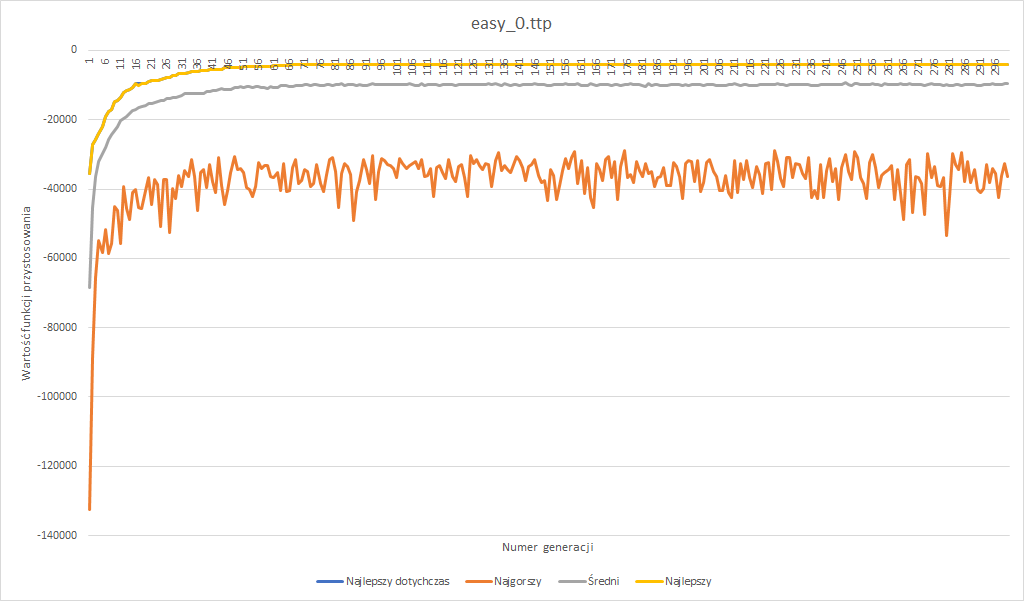
\includegraphics[width=1\linewidth]{easy0.png}
		\caption{Przykładowy przebieg metody dla instancji easy\_0}
		\label{fig:easy0}
	\end{figure}
	\begin{center}
		$\mu = -5168.9$
		\\$\sigma =719.7$
	\end{center}


	\subsection{Problem easy\_1.ttp}
	\begin{figure}[H]
		\centering
		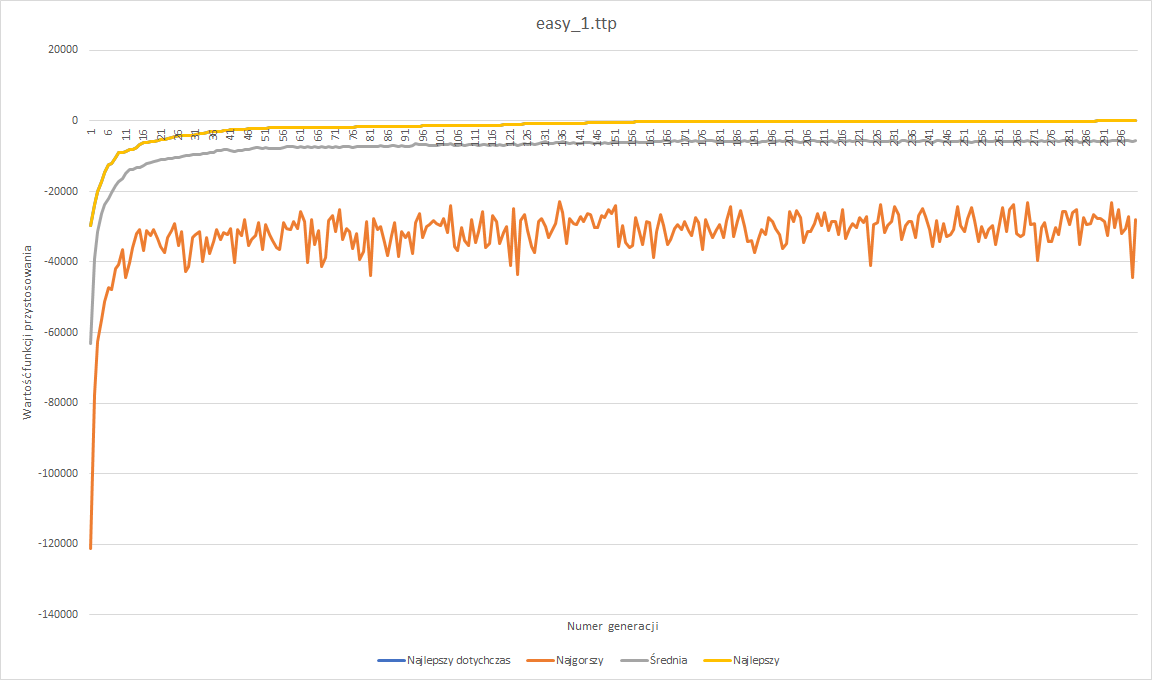
\includegraphics[width=1\linewidth]{easy1.png}
		\caption{Przykładowy przebieg metody dla instancji easy\_1}
		\label{fig:easy1}
	\end{figure}
	\begin{center}
		$\mu = 613.4$
		\\$\sigma =794.64$
	\end{center}


	\subsection{Problem medium\_0.ttp}
	\begin{figure}[H]
		\centering
		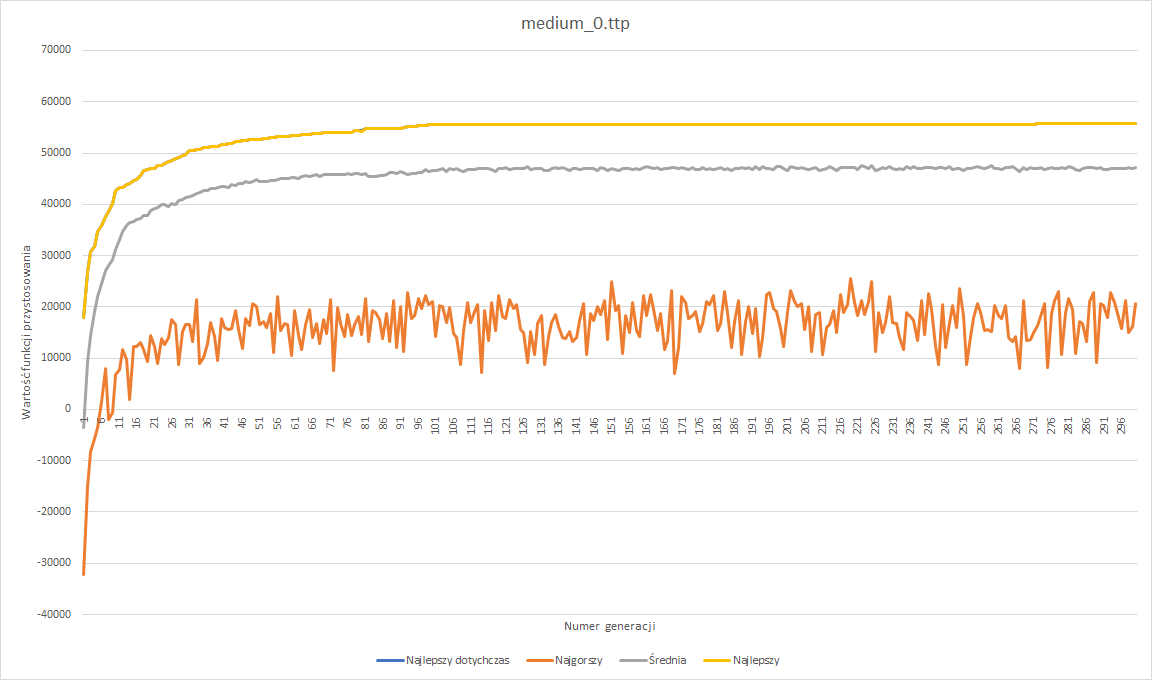
\includegraphics[width=1\linewidth]{medium0.png}
		\caption{Przykładowy przebieg metody dla instancji medium\_0}
		\label{fig:medium0}
	\end{figure}
	\begin{center}
		$\mu = 57284.8$
		\\$\sigma = 1046.99$
	\end{center}


	\subsection{Problem medium\_1.ttp}
	\begin{figure}[H]
		\centering
		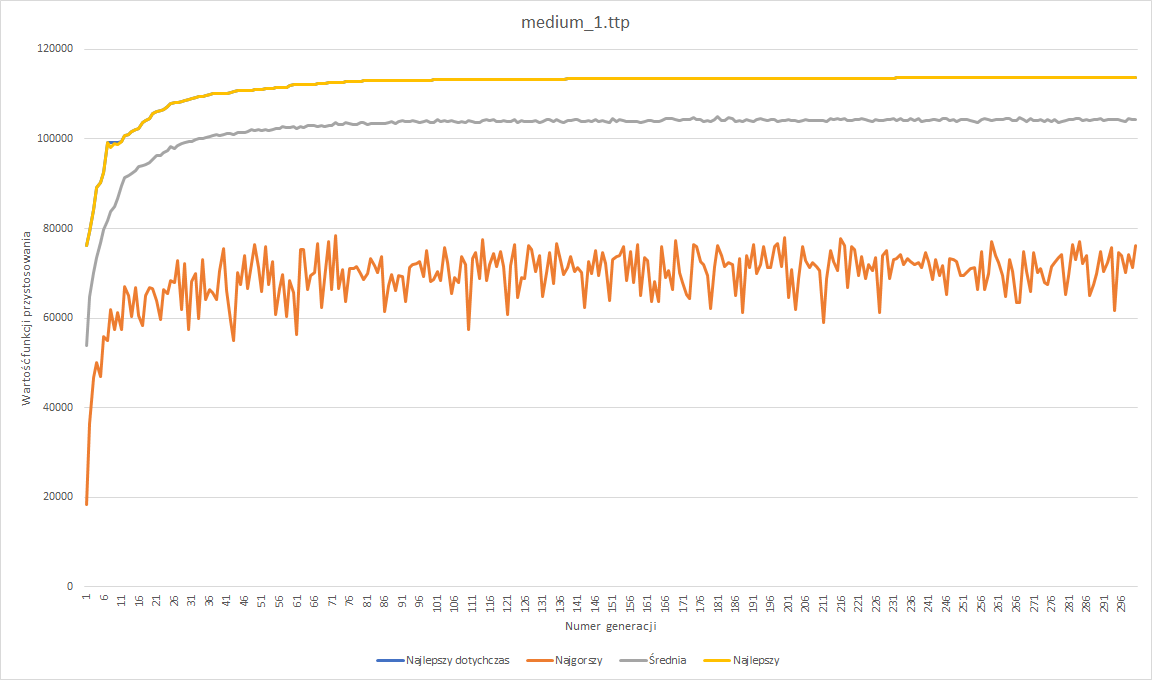
\includegraphics[width=1\linewidth]{medium1.png}
		\caption{Przykładowy przebieg metody dla instancji medium\_1}
		\label{fig:medium1}
	\end{figure}
	\begin{center}
		$\mu = 113726.1$
		\\$\sigma = 1692.03$
	\end{center}


	\subsection{Problem hard\_0.ttp}
	\begin{figure}[H]
		\centering
		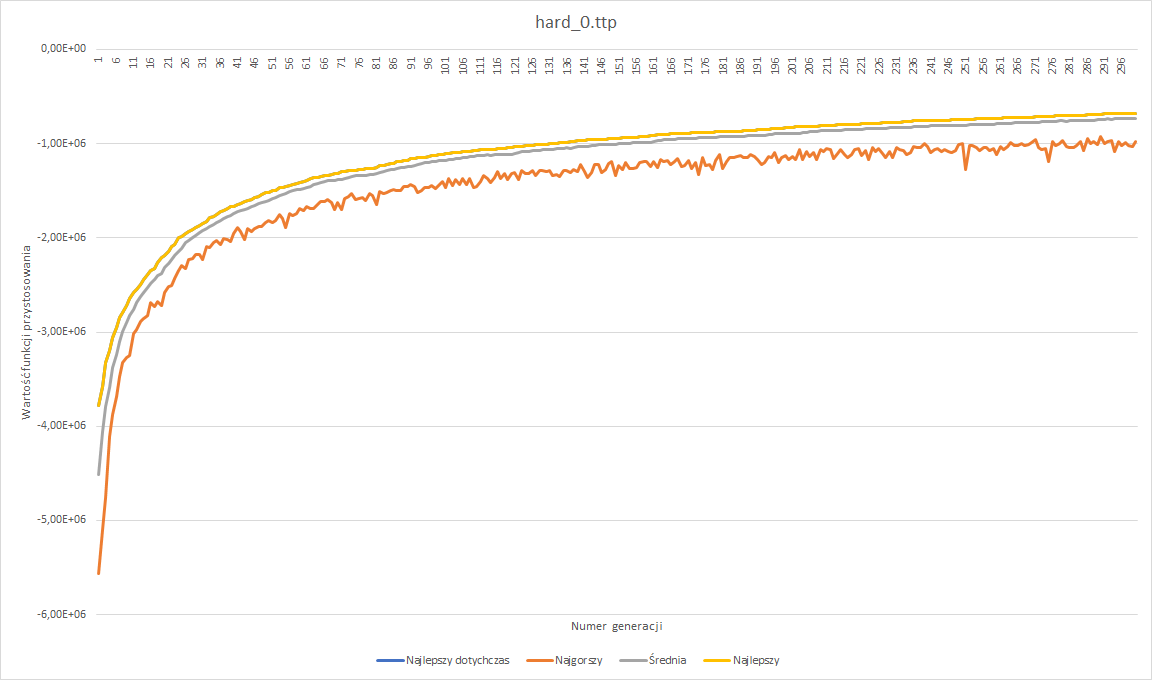
\includegraphics[width=1\linewidth]{hard0.png}
		\caption{Przykładowy przebieg metody dla instancji hard\_0}
		\label{fig:hard0}
	\end{figure}
	\begin{center}
		$\mu = -713010.9$
		\\$\sigma = 43227.52$
	\end{center}

	\subsection{Wnioski}
	Z powyższych wykresów można wnioskować, że algorytm genetyczny działa poprawnie. Widać że wartość średnia jest oddalona od najlepszego rozwiązania, a wartość przystosowania najgorszego osobnika w populacji jest znacząco oddalona od średniej, co może oznaczać, że przestrzeń rozwiązań jest poprawnie eksplorowana. Z drugiej strony można zauważyć, że dla czterech pierwszych instancji problemu TTP, algorytm zdaje się utykać i nie znajdować lepszych rozwiązań po mniejszej liczbie iteracji niż została przewidziana. Być może lepiej byłoby zatem zmniejszyć ten parametr i uruchomić metodę więcej razy lub inaczej dobrać wartości innych parametrów.
	Z kolei na wykresie przebiegu dla instancji hard\_0 widać, że nawet po upływie 300 generacji, dalej zauważalna jest tendencja wzrostowa, co oznacza że dobrze byłoby próbować szukać rozwiązania dłużej.


	\section{Badanie wpływu parametrów metody na \mbox{wyniki} działania}
	W tej sekcji przedstawione zostaną wyniki badań dotyczących wpływu wartości poszczególnych parametrów na wyniki działania algorytmu genetycznego. Dla każdej wartości parametru zostało wykonane 10 uruchomień.
	\subsection{Wpływ prawdopodobieństwa mutacji}
	Pierwszy parametr, który zostanie omówiony to prawdopodobieństwo mutacji - $p_m$. Badanie zostało przeprowadzone dla problemu medium\_0.ttp, a wartości innych parametrów zostały ustawione następująco:
	\begin{itemize}
		\item $gen = 100$,
		\item $pop\_size = 100$,
		\item $p_x = 0.8$,
		\item $tour = 10$.
	\end{itemize}

	\begin{figure}[H]
		\centering
		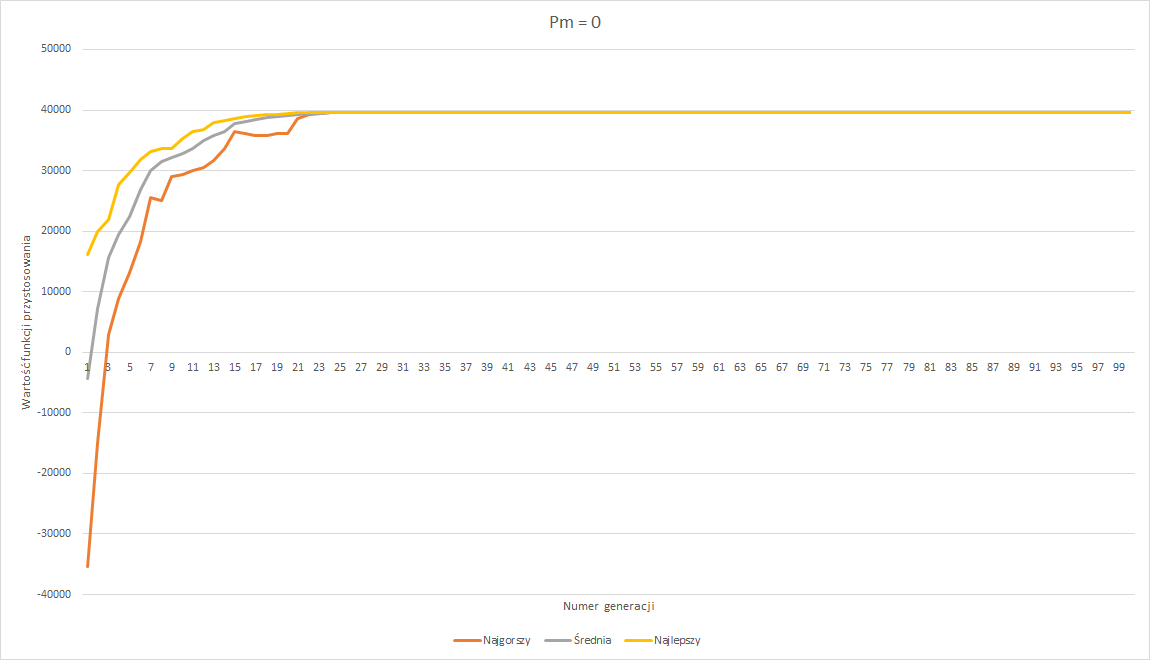
\includegraphics[width=1\linewidth]{pm0.png}
		\caption{Przykładowy przebieg dla $p_m=0$}
		\label{fig:pm0}
	\end{figure}
	
	
	\begin{figure}[H]
		\centering
		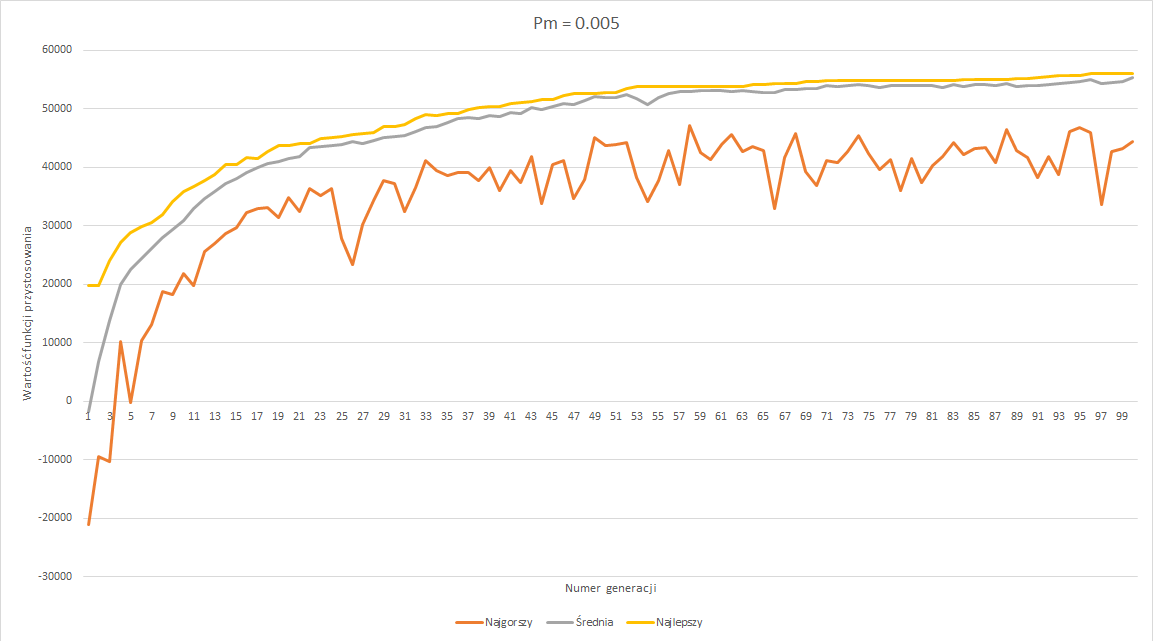
\includegraphics[width=1\linewidth]{pm0005.png}
		\caption{Przykładowy przebieg dla $p_m=0.005$}
		\label{fig:pm0005}
	\end{figure}

	\begin{figure}[H]
		\centering
		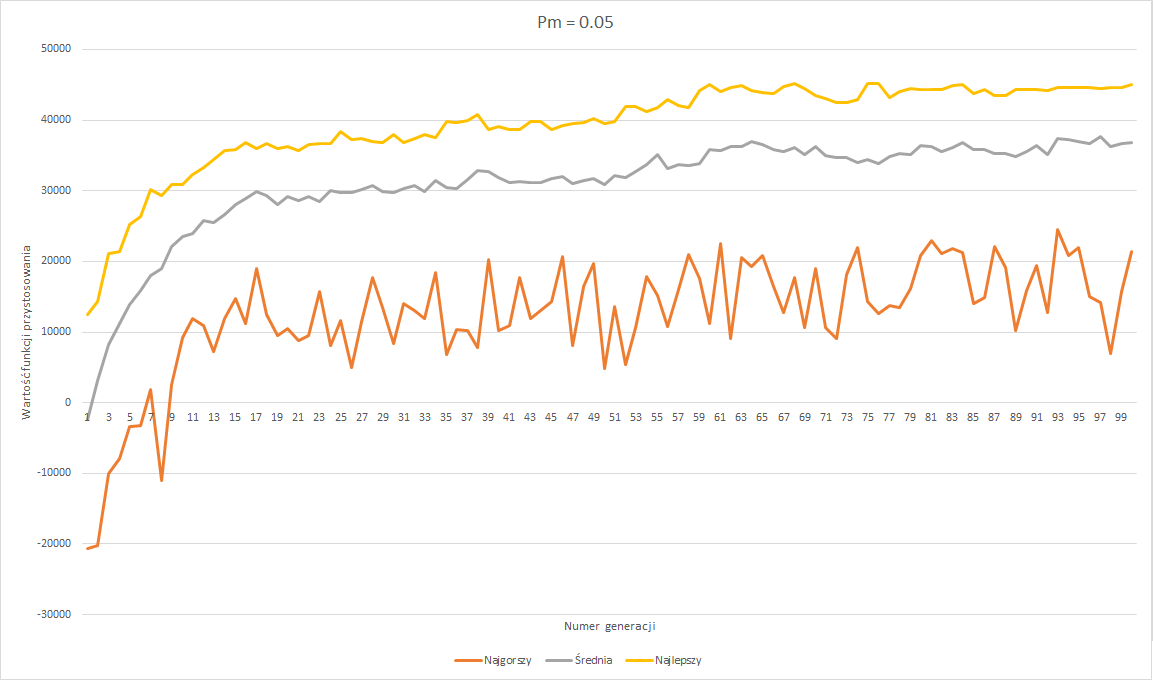
\includegraphics[width=1\linewidth]{pm005.png}
		\caption{Przykładowy przebieg dla $p_m=0.05$}
		\label{fig:pm005}
	\end{figure}
	

	\begin{figure}[H]
	\centering
	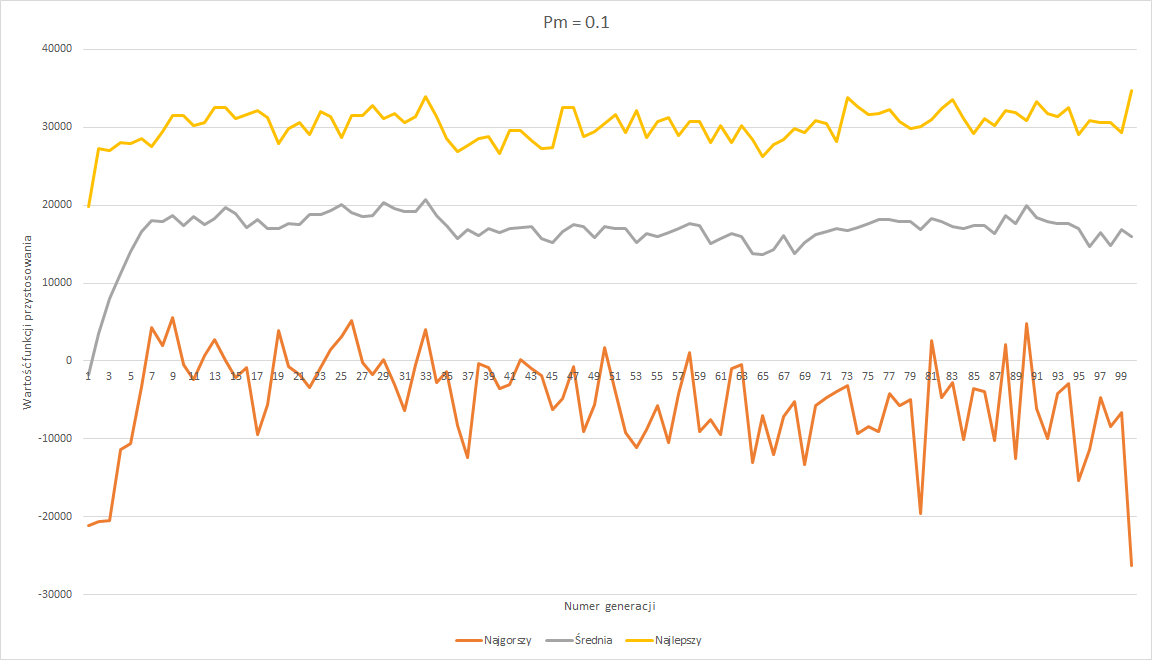
\includegraphics[width=1\linewidth]{pm01.png}
	\caption{Przykładowy przebieg dla $p_m=0.1$}
	\label{fig:pm01}
	\end{figure}

	\begin{figure}[H]
		\centering
		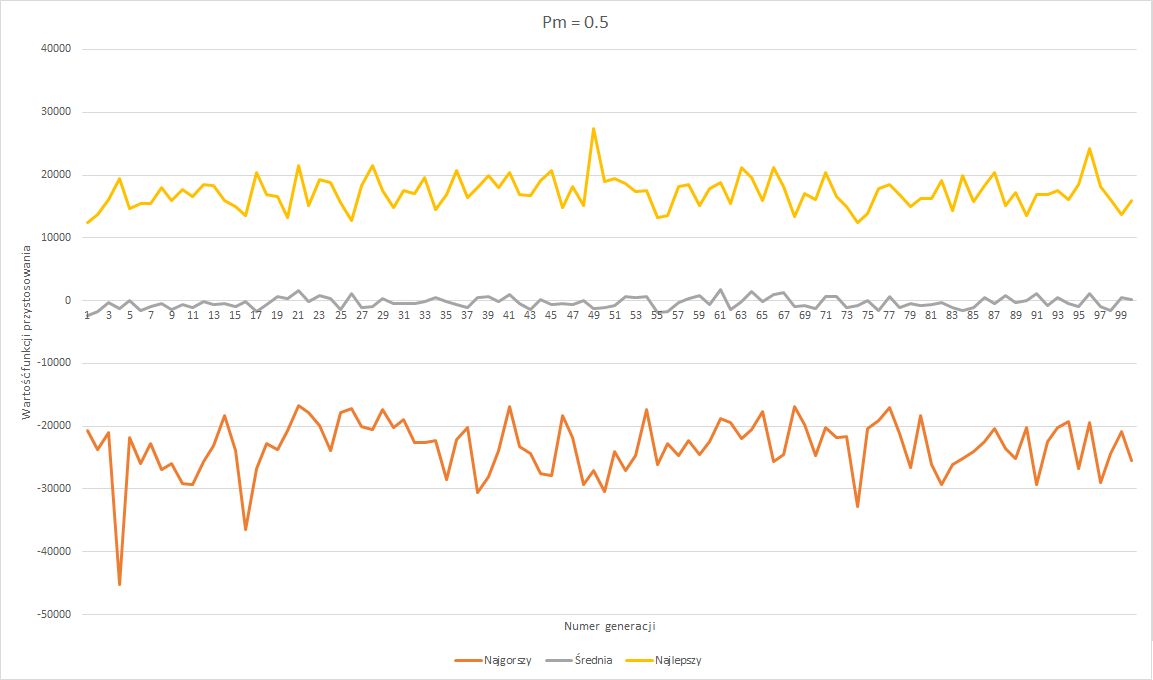
\includegraphics[width=1\linewidth]{pm05.png}
		\caption{Przykładowy przebieg dla $p_m=0.5$}
		\label{fig:pm05}
	\end{figure}

	\begin{figure}[H]
		\centering
		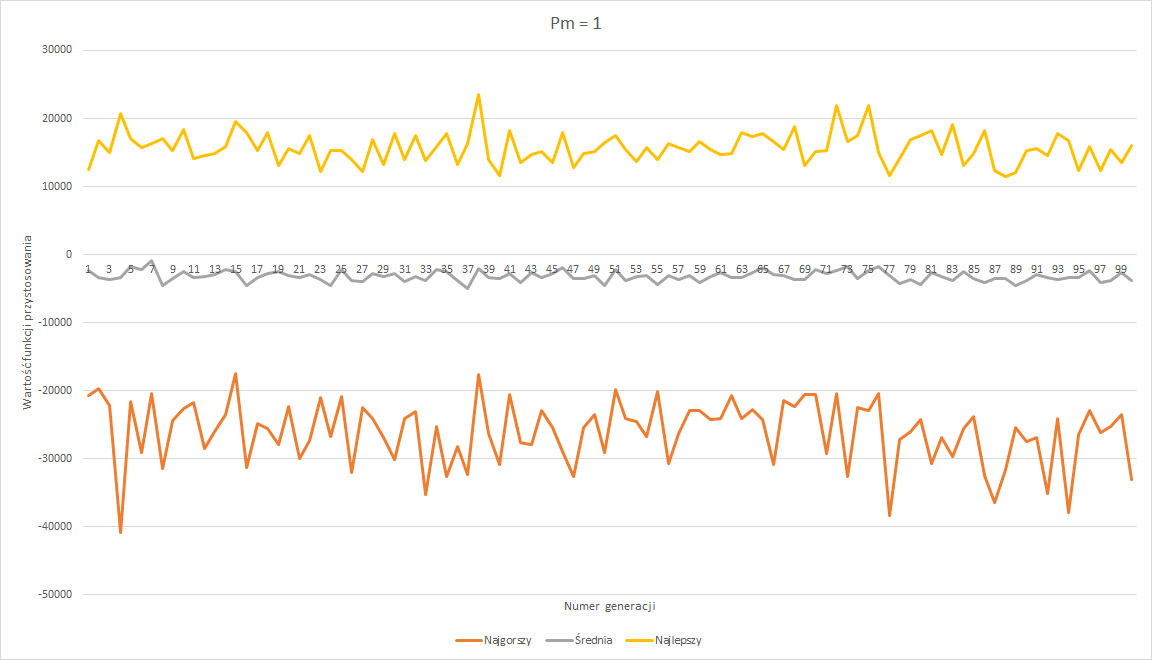
\includegraphics[width=1\linewidth]{pm1.png}
		\caption{Przykładowy przebieg dla $p_m=1$}
		\label{fig:pm1}
	\end{figure}
	
	\begin{table}[H]
		\begin{center}
			\begin{tabular}{ |c|c|c| } 
				\hline
				$p_m$ & $\mu$ & $\sigma$ \\ 
				\hline
				0 & 38837.3 & 4054.36 \\ 
				0.005 & \textbf{53087.7} & 1900.79 \\ 
				0.05 & 45279.2 & 1644.11 \\ 
				0.1 & 36578.1 & 1425.52 \\ 
				0.5 & 25012.4 & 1342.05 \\ 
				1 & 23004.6 & 1202.17 \\ 
				\hline
			\end{tabular}
			\caption{Średnia wartość i odchylenie standardowe funkcji przystosowania najlepszego znalezionego osobnika, dla różnych wartości parametru $p_m$.}
			\label{tab:mut}
		\end{center}
	\end{table}
	
	\paragraph{Wnioski}
	Jak widać na rysunku \ref{fig:pm0} przy prawdopodobieństwie mutacji = 0, po pewnej liczbie iteracji, cała populacja zbiega do jednego punktu. Brakuje źródła różnorodności. Z kolei już na rysunku \ref{fig:pm005} i w tabeli \ref{tab:mut} widać, że prawdopodobieństwo mutacji większe od 0.05 zaczyna stopniowo pogarszać jakość wyników. Przy zbyt dużych wartościach tego prawdopodobieństwa przeszukiwanie staje się zbyt losowe. Przy tak zdefiniowanym operatorze mutacji, dla problemu medium\_0, wartość około pomiędzy $0.005$, a $0.015$ zdaje się być odpowiednia.
	
	\subsection{Wpływ prawdopodobieństwa krzyżowania}
	Kolejny parametr, który zostanie omówiony to prawdopodobieństwo krzyżowania $p_x$. Badanie również zostało przeprowadzone na problemie medium\_0, a ustalone wartości parametrów wyglądały następująco:
	\begin{itemize}
		\item $gen = 100$,
		\item $pop\_size = 100$,
		\item $p_m = 0.015$,
		\item $tour = 10$.
	\end{itemize}

	\begin{figure}[H]
		\centering
		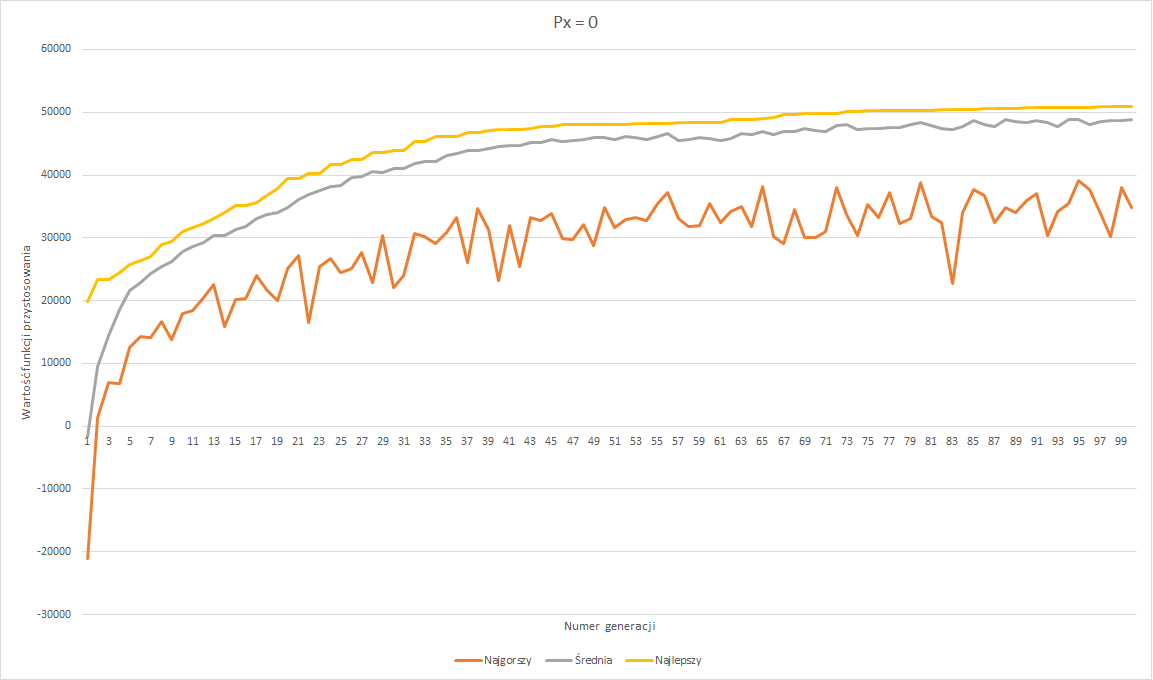
\includegraphics[width=1\linewidth]{cross0.png}
		\caption{Przykładowy przebieg dla $p_x=0$}
		\label{fig:px0}
	\end{figure}
	
	
	\begin{figure}[H]
		\centering
		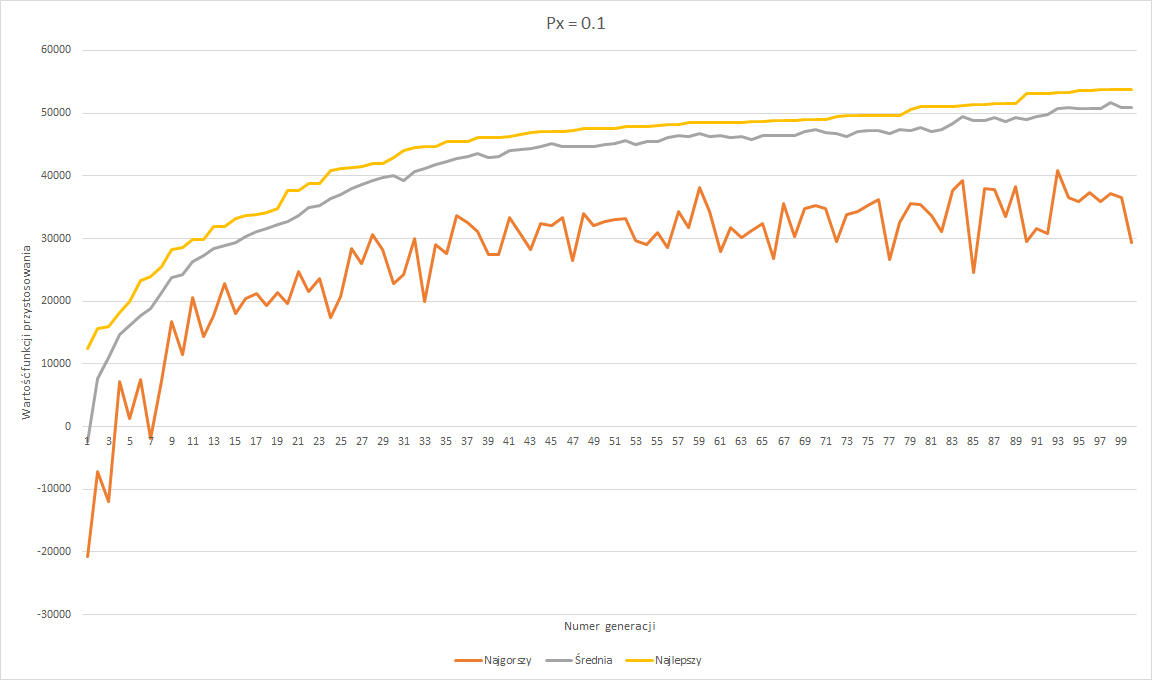
\includegraphics[width=1\linewidth]{cross01.png}
		\caption{Przykładowy przebieg dla $p_x=0.1$}
		\label{fig:px01}
	\end{figure}
	
	\begin{figure}[H]
		\centering
		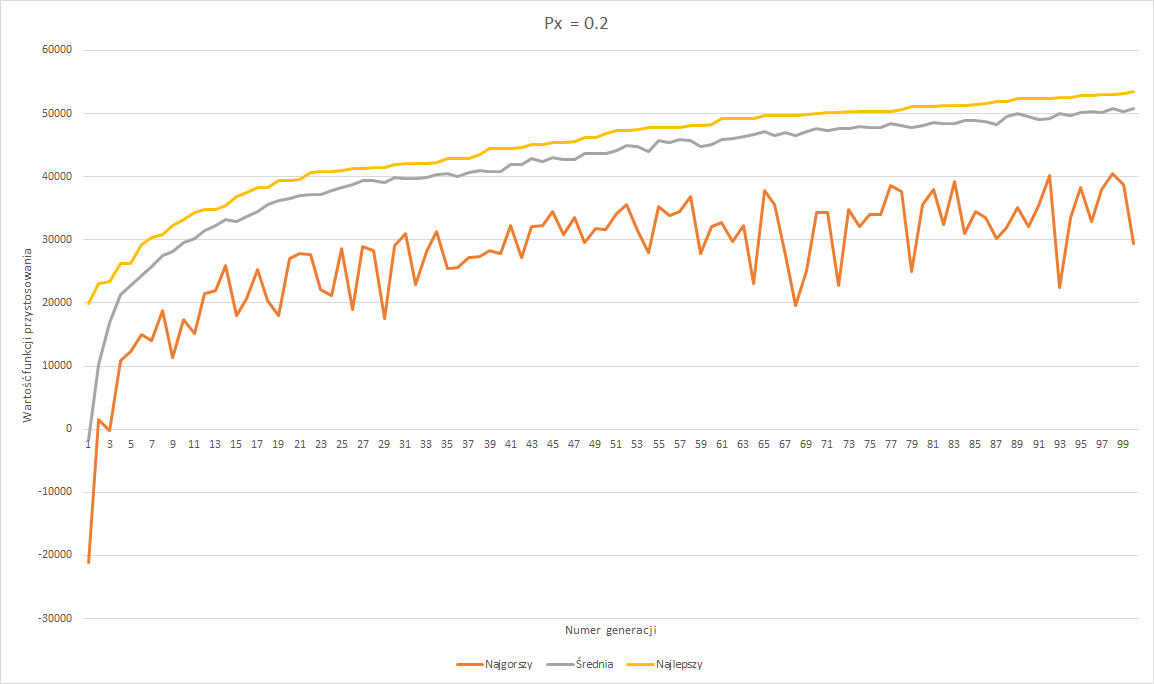
\includegraphics[width=1\linewidth]{cross02.png}
		\caption{Przykładowy przebieg dla $p_x=0.2$}
		\label{fig:px02}
	\end{figure}
	
	\begin{figure}[H]
		\centering
		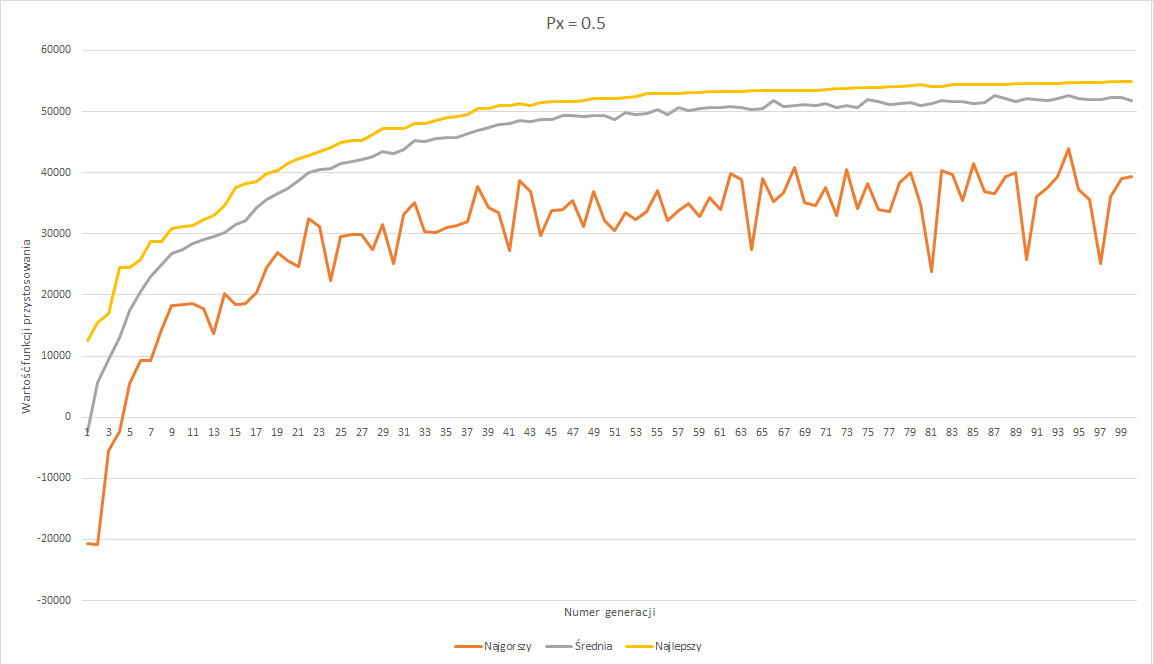
\includegraphics[width=1\linewidth]{cross05.png}
		\caption{Przykładowy przebieg dla $p_x=0.5$}
		\label{fig:px05}
	\end{figure}
	
	\begin{figure}[H]
		\centering
		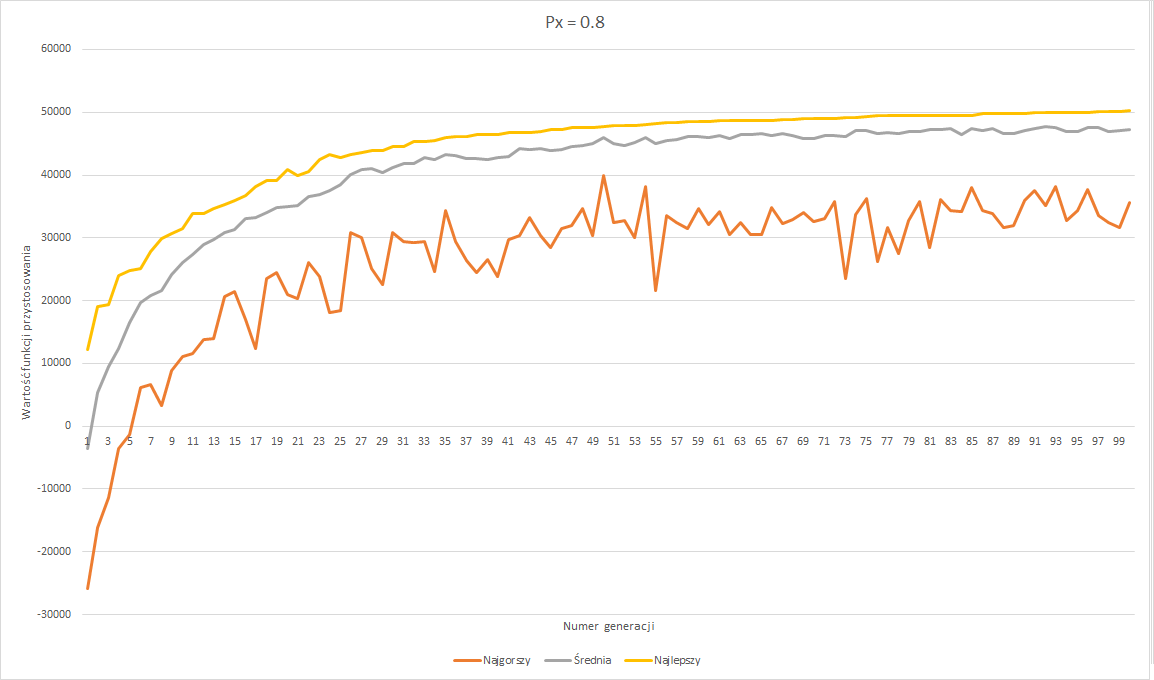
\includegraphics[width=1\linewidth]{cross08.png}
		\caption{Przykładowy przebieg dla $p_x=0.8$}
		\label{fig:px08}
	\end{figure}
	
	\begin{figure}[H]
		\centering
		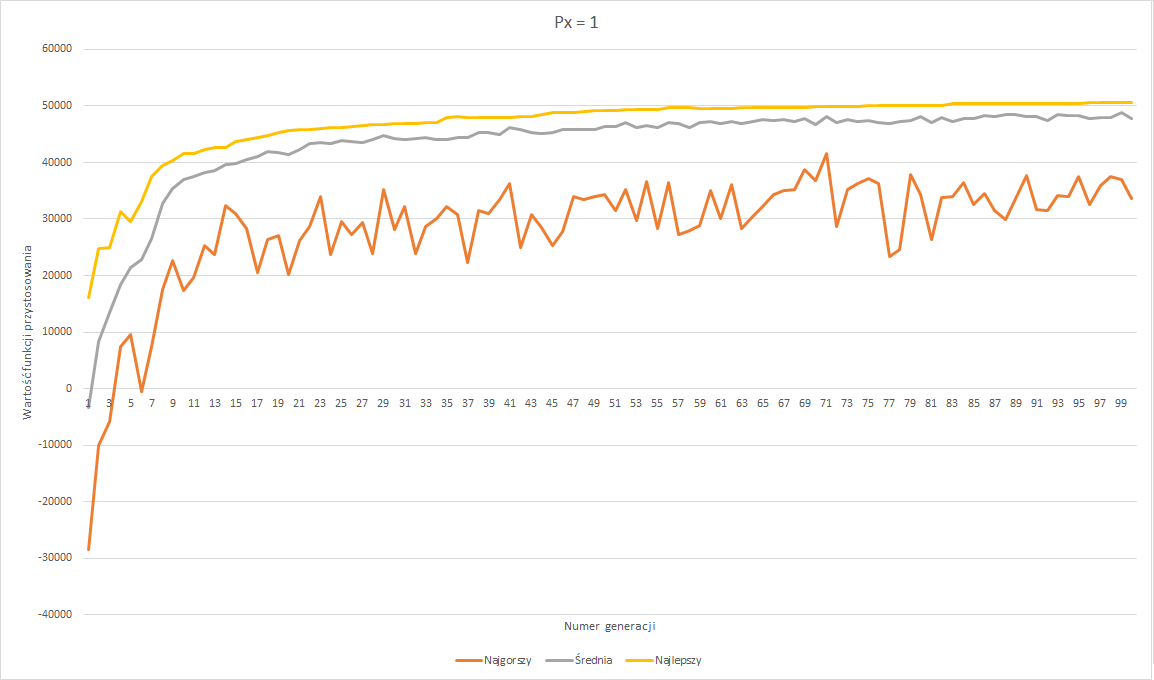
\includegraphics[width=1\linewidth]{cross1.png}
		\caption{Przykładowy przebieg dla $p_x=1$}
		\label{fig:px1}
	\end{figure}

	\begin{table}[H]
		\begin{center}
			\begin{tabular}{ |c|c|c| } 
				\hline
				$p_x$ & $\mu$ & $\sigma$ \\ 
				\hline
				0 & 51535.7 & 984.14 \\ 
				0.1 & 52316.9 & 1982.64 \\ 
				0.2 & 51933.6 & 1498.61 \\ 
				0.5 & 52560.9 & 1942.67 \\ 
				0.8 & 52271.5 & 1604.25 \\ 
				1 & 53329.6 & 1942.71 \\ 
				\hline
			\end{tabular}
			\caption{Średnia wartość i odchylenie standardowe funkcji przystosowania najlepszego znalezionego osobnika, dla różnych wartości parametru $p_x$.}
			\label{tab:cross}
		\end{center}
	\end{table}
	
	\paragraph{Wnioski}
	Wnioskowanie na temat wpływu prawdopodobieństwa krzyżowania na jakość znajdowanych rozwiązań, nie jest w przypadku tego problemu tak oczywista jak w przypadku operatora mutacji. Na podstawie uzyskanych wyników nie da się łatwo stwierdzić jaka powinna być ta wartość, aby otrzymywane wyniki były jak najlepsze.
	
	\subsection{Wpływ rozmiaru populacji}
	W następnej kolejności zostaną omówione wyniki badań nad wpływem rozmiaru populacji na jakość znajdowanych rozwiązań. To badanie zostało przeprowadzone na instancji hard\_0. Ze względu na silną korelację parametrów $pop\_size$ i $tour$, w tym badaniu były zmieniane wartości ich obu. Wynika to z faktu że stosunek tych dwóch wartości steruje presją selekcyjną. Wartości reszty parametrów zostały ustalone następująco:
	\begin{itemize}
		\item $gen = 100$,
		\item $p_m = 0.005$,
		\item $p_x = 0.8$.
	\end{itemize}
	
	\begin{figure}[H]
		\centering
		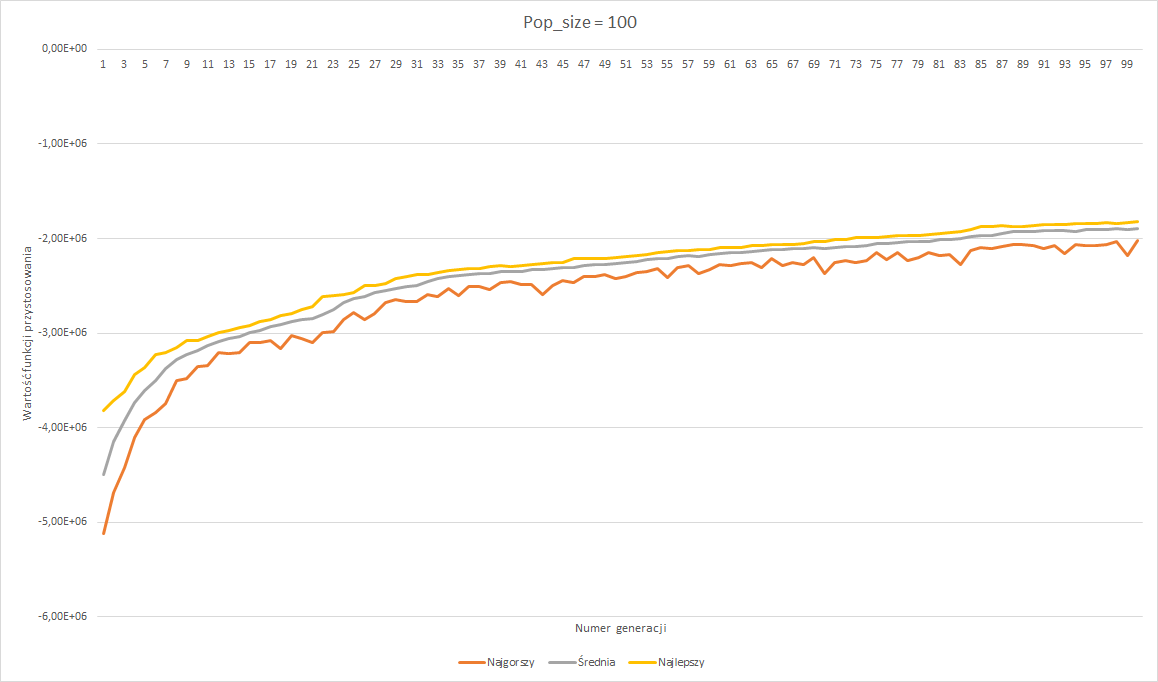
\includegraphics[width=1\linewidth]{popsize100.png}
		\caption{Przykładowy przebieg dla $pop\_size=100$}
		\label{fig:pop100}
	\end{figure}
	
	
	\begin{figure}[H]
		\centering
		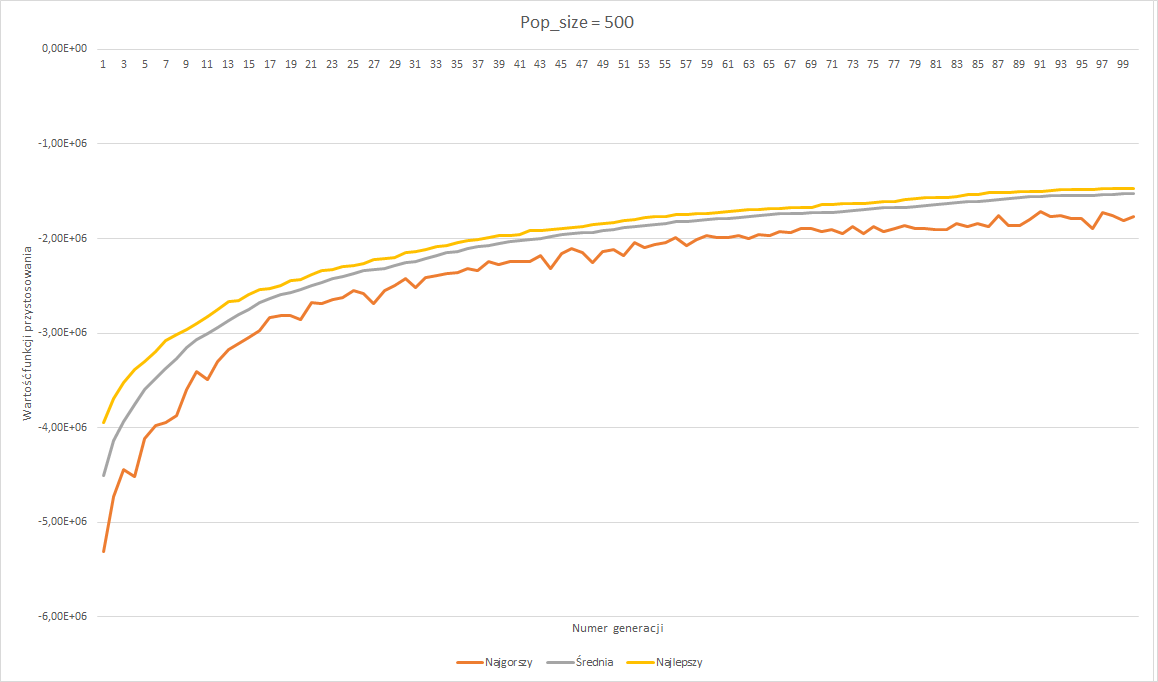
\includegraphics[width=1\linewidth]{popsize500.png}
		\caption{Przykładowy przebieg dla $pop\_size=500$}
		\label{fig:pop500}
	\end{figure}
	
	\begin{figure}[H]
		\centering
		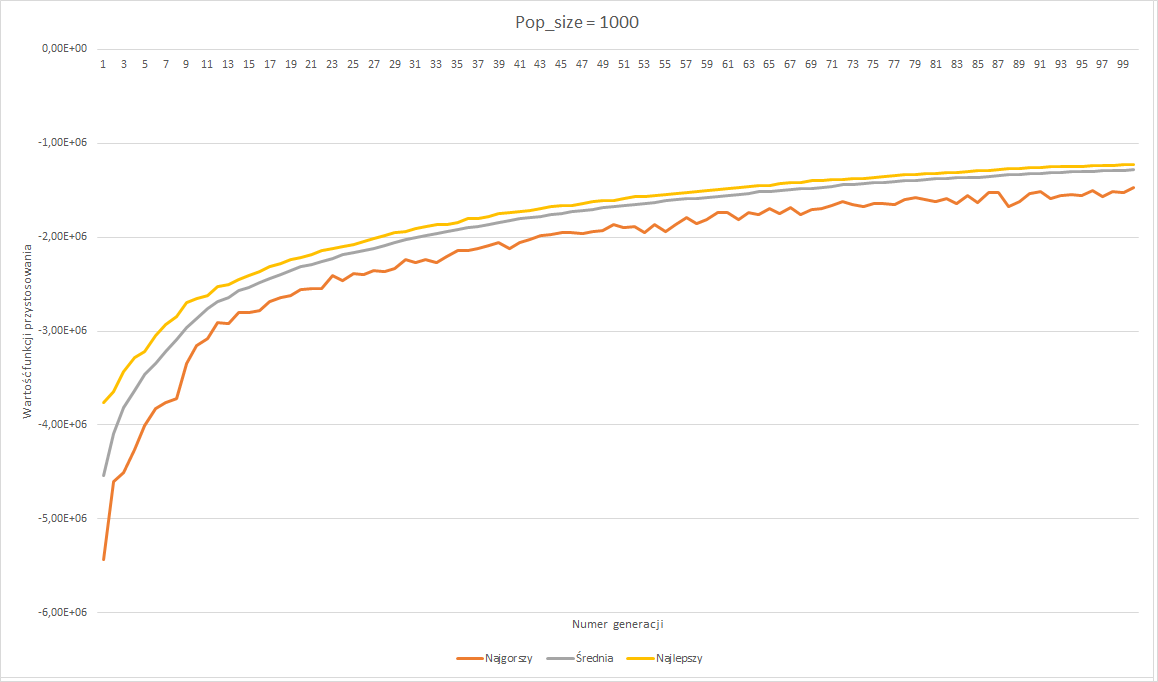
\includegraphics[width=1\linewidth]{popsize1000.png}
		\caption{Przykładowy przebieg dla $pop\_size=1000$}
		\label{fig:pop1000}
	\end{figure}

	\begin{table}[H]
		\begin{center}
			\begin{tabular}{ |c|c|c| } 
				\hline
				$pop\_size$ & $\mu$ & $\sigma$ \\ 
				\hline
				100 & -1843672 & 66598,53 \\ 
				500 & -1401129 & 49426,29 \\ 
				1000 & -1194559 & 17964,83 \\ 
				\hline
			\end{tabular}
			\caption{Średnia wartość i odchylenie standardowe funkcji przystosowania najlepszego znalezionego osobnika, dla różnych wartości parametru $pop\_size$.}
			\label{tab:pop}
		\end{center}
	\end{table}
	
	\paragraph{Wnioski}
	Z tabeli \ref{tab:pop} dość dobrze widać, jak istotnym parametrem jest wielkość populacji. Dla problemu hard\_0, przy zwiększaniu wartości tego parametru znacząco poprawia się zarówno średnia jak i odchylenie standardowe. Wielkość populacji ma bezpośredni wpływ na liczbę przeglądanych przez algorytm rozwiązań.
	
	
	\subsection{Wpływ liczby pokoleń}
	Ostatnim omawianym parametrem będzie liczba pokoleń. To badanie, tak jak poprzednie, zostało przeprowadzone na problemie hard\_0. Wartości parametrów zostały ustalone następująco:
	\begin{itemize}
		\item $pop\_size = 500$
		\item $p_m = 0.005$,
		\item $p_x = 0.8$,
		\item $tour = 25$.
	\end{itemize}
	
	\begin{figure}[H]
		\centering
		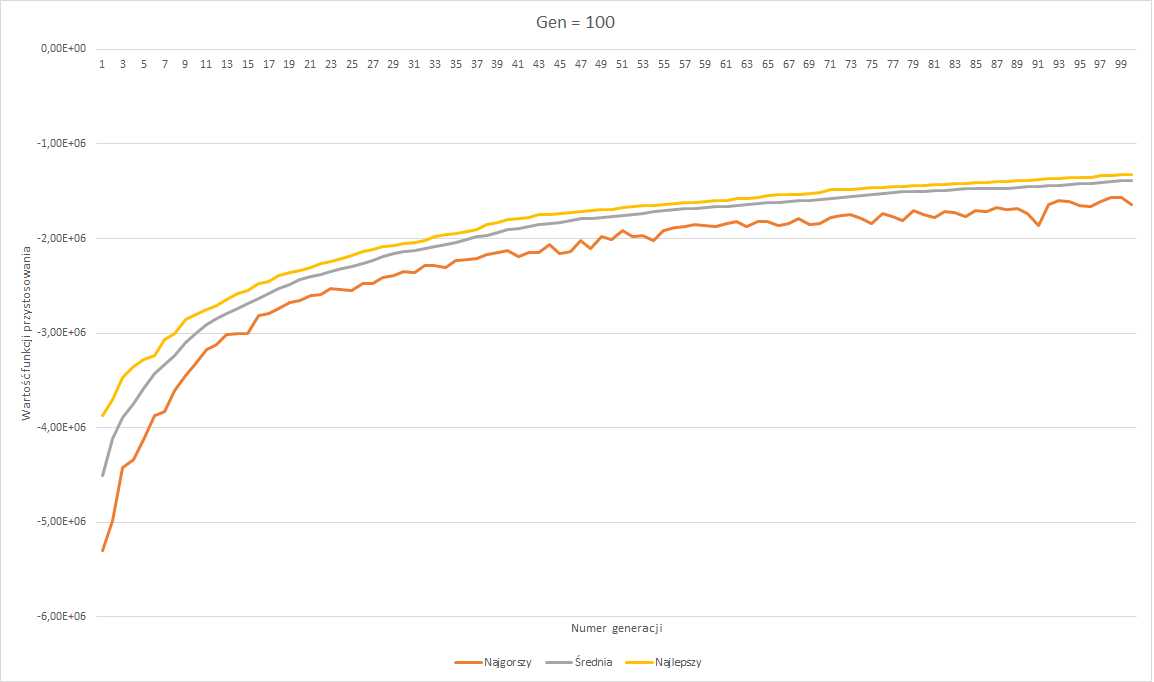
\includegraphics[width=1\linewidth]{gen100.png}
		\caption{Przykładowy przebieg dla $gen=100$}
		\label{fig:gen100}
	\end{figure}
	
	
	\begin{figure}[H]
		\centering
		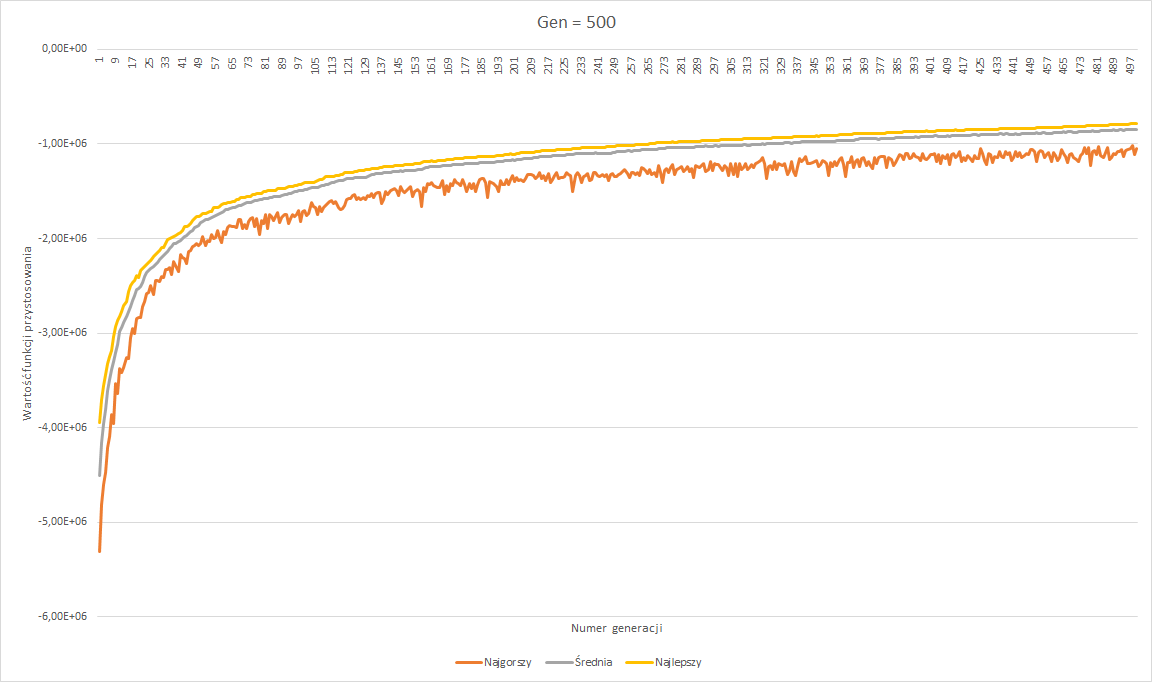
\includegraphics[width=1\linewidth]{gen500.png}
		\caption{Przykładowy przebieg dla $gen=500$}
		\label{fig:gen500}
	\end{figure}
	
	\begin{figure}[H]
		\centering
		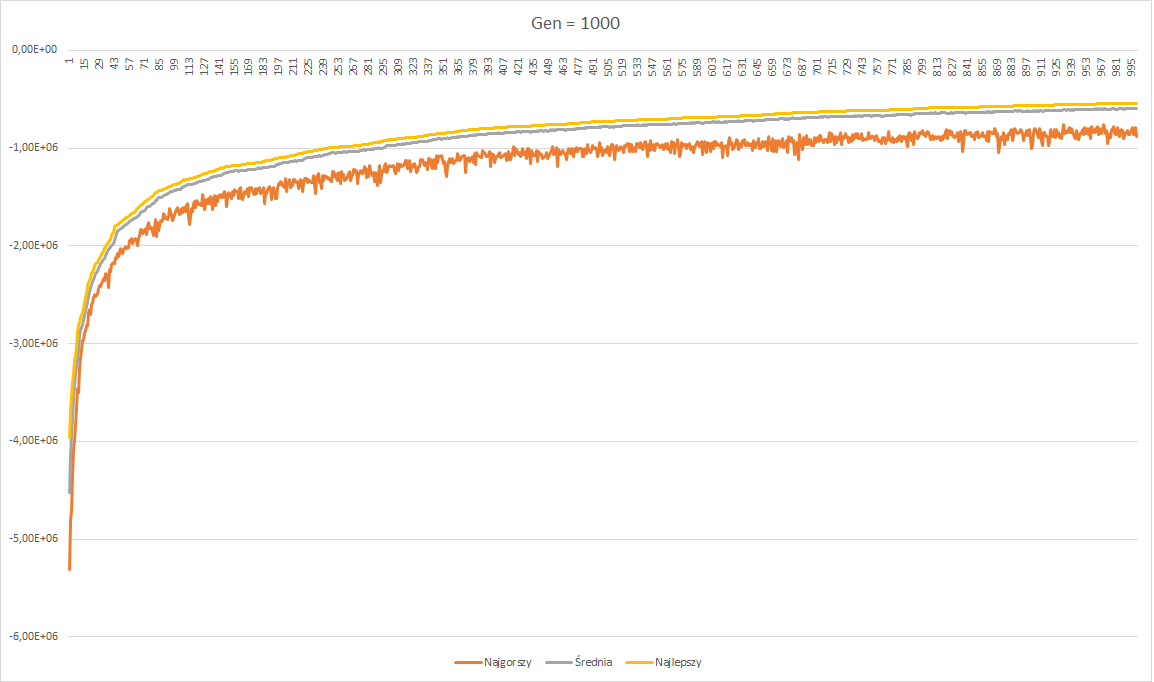
\includegraphics[width=1\linewidth]{gen1000.png}
		\caption{Przykładowy przebieg dla $gen=1000$}
		\label{fig:gen1000}
	\end{figure}
	
	\begin{table}[H]
		\begin{center}
			\begin{tabular}{ |c|c|c| } 
				\hline
				$pop\_size$ & $\mu$ & $\sigma$ \\ 
				\hline
				100 & -1390237,0 & 57115,43 \\ 
				500 & -741901,7 & 44242,51 \\ 
				1000 & -527889,9 & 47903,73 \\ 
				\hline
			\end{tabular}
			\caption{Średnia wartość i odchylenie standardowe funkcji przystosowania najlepszego znalezionego osobnika, dla różnych wartości parametru $gen$.}
			\label{tab:gen}
		\end{center}
	\end{table}
	
	\paragraph{Wnioski}
	Z otrzymanych wyników dobrze widać, że tak jak wielkość populacji, liczba generacji ma bardzo duży wpływ na jakość znalezionych rozwiązań.
	
	\section{Badanie wpływu selekcji na skuteczność \mbox{algorytmu} genetycznego}
	W tej sekcji omówione zostaną wyniki badań wpływu dwóch rodzajów selekcji na skuteczność algorytmu genetycznego. Oba zostaną przeprowadzone na problemie medium\_0 z parametrami:
	\begin{itemize}
		\item $gen = 300$
		\item $pop\_size = 100$
		\item $p_m = 0.015$,
		\item $p_x = 0.8$,
		\item $tour = 10$.
	\end{itemize}

	\begin{figure}[H]
		\centering
		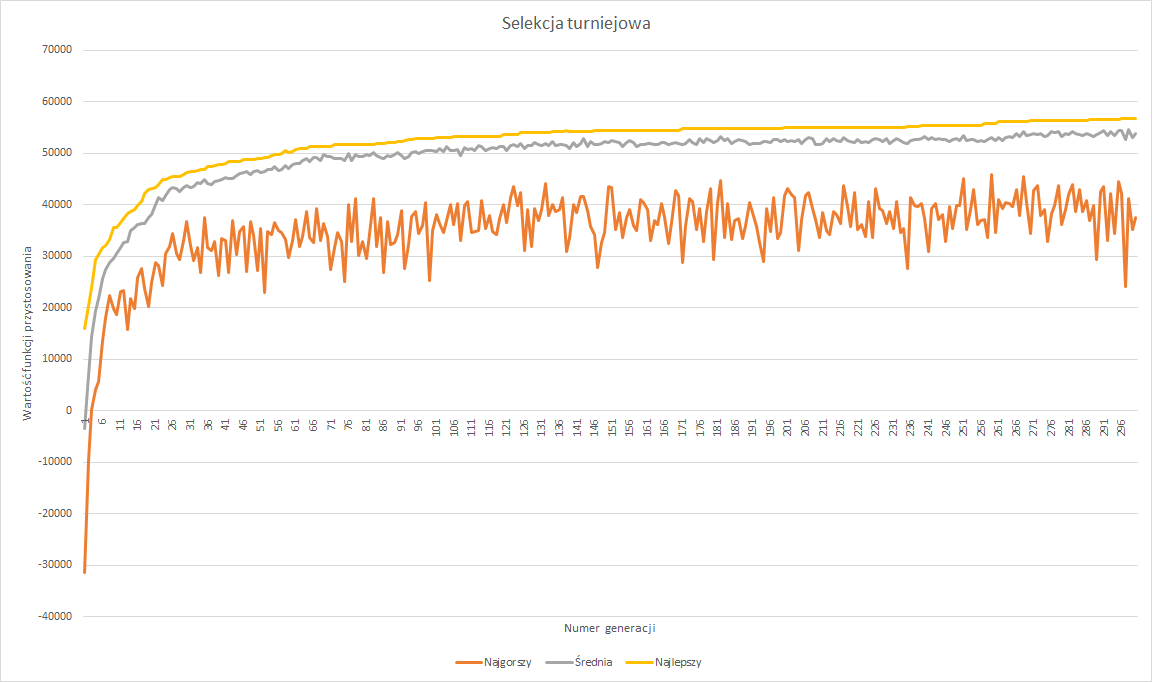
\includegraphics[width=1\linewidth]{tour.png}
		\caption{Przykładowy przebieg dla selekcji turniejowej}
		\label{fig:tour}
	\end{figure}

	\begin{figure}[H]
		\centering
		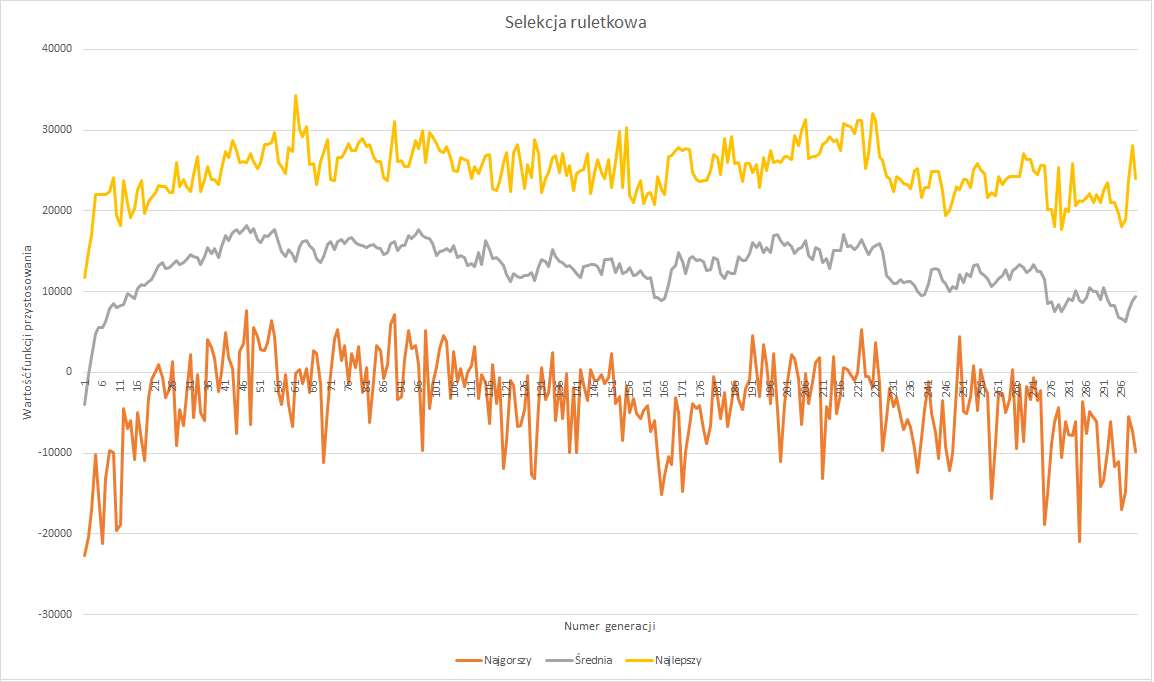
\includegraphics[width=1\linewidth]{roulette.png}
		\caption{Przykładowy przebieg dla selekcji ruletkowej}
		\label{fig:roulette}
	\end{figure}

	\begin{table}[H]
		\begin{center}
			\begin{tabular}{ |c|c|c| } 
				\hline
				Rodzaj selekcji & $\mu$ & $\sigma$ \\ 
				\hline
				turniej & 56370.1 & 1264.43 \\ 
				ruletka & 32256.8 & 988.66 \\ 
				\hline
			\end{tabular}
			\caption{Średnia wartość i odchylenie standardowe funkcji przystosowania najlepszego znalezionego osobnika, dla różnych rodzajów selekcji.}
			\label{tab:gen}
		\end{center}
	\end{table}
	\paragraph{Wnioski}	
	Z rysunków \ref{fig:tour} i \ref{fig:roulette} widać, że selekcja turniejowa daje zdecydowanie lepsze rezultaty niż selekcja ruletkowa. Ruletka bez żadnych modyfikacji zdaje się być zbyt losowa i nie dawać tak dobrze ukierunkowanego przeszukiwania jak turniej.
	
	\section{Porównanie skuteczności algorytmu genetycznego z wynikami metod nieewolucyjnych}
	Do porównania zostały wybrane następujące algorytmy nieewolucyjne:
	\begin{itemize}	
		\item przeszukiwanie losowe,
		\item algorytm wspinaczkowy (\textit{Hill Climber}),
		\item algorytm zachłanny.
	\end{itemize}
	
	\begin{table}[H]
		\begin{center}
			\begin{tabular}{ |c|c|c|c|c|c| } 
				\hline
				Algorytm & easy\_0 & easy\_1 & medium\_0 & medium\_1 & hard\_0 \\ 
				\hline
				GA & -5168.9 & \textbf{613.4} & 57284.8 & 113726.1 & -713010 \\ 
				RS & -28520.7 & -22798.6 & 26485.6 & 83114.4 & -3581490 \\ 
				HC & \textbf{-4397,3} & 1517.1 & \textbf{58150.2} & \textbf{115924} & n/a \\ 
				Zachłanny & -18206 & -19556.3 & 47730.8 & 105551 & \textbf{61718.2} \\ 
				\hline
			\end{tabular}
			\caption{Zestawienie jakości rozwiązań problemów znalezionych przy pomocy poszczególnych algorytmów.}
			\label{tab:nev}
		\end{center}
	\end{table}
	
	\paragraph{Wnioski}
	Algorytm przeszukiwania losowego w żadnym stopniu nie sprawdza się do tak ogromnych przestrzeni rozwiazań. Algorytm wspinaczkowy z kolei, znalazł najlepsze rozwiązania dla 3 z 5 problemów. Posiada on jednak jedną zasadniczą wadę - wymaga ogromnej liczby ewaluacji funkcji celu. Warte uwagi jest również to, że algorytm zachłanny znalazł najlepsze rozwiązanie problemu hard\_0. Jego dużą zaletą jest to, że do problemu TSP wymaga tylko $N$ ewaluacji funkcji celu, gdzie N jest liczbą możliwych miast początkowych.\\
	Bardzo istotny jest również fakt, że algorytm genetyczny znalazł rozwiązania niewiele gorsze niż algorytm wspinaczkowy, a osiągnął to dużo mniejszym kosztem. Prawdopodobnie gdyby dobrać lepsze operatory genetyczne i przeprowadzić dokładniejsze strojenie parametrów, algorytm genetyczny poradziłby sobie najlepiej we wszystkich problemach.
	\section{Podsumowanie}
	Algorytm genetyczny jest bardzo dobrą metodą optymalizacji do problemów, w których występują ogromne przestrzenie rozwiązań. Pozwala on znajdować dobre jakościowo rozwiązania dużo mniejszym kosztem niż inne metody optymalizacji. Jego największą wadą jest duża liczba silnie powiązanych ze sobą parametrów, które do każdego problemu należy dobrać osobno, tak aby algorytm działał dobrze.
\end{document}